% Generated by html2tex: Version Aud2.8 of November 14th, 2017.
% Written by F.J. Faase.  http://www.iwriteiam.nl/
% Adapted by J.K. Crook.  http://audacityteam.org/

\documentclass[twocolumn]{book}
%\usepackage{multicol}
\usepackage[latin1]{inputenc}
%\usepackage[utf8]{inputenc} 
\usepackage[T1]{fontenc}
\usepackage[english]{babel}
\usepackage{amsmath}
\usepackage{amssymb,amsfonts,textcomp}
\usepackage{color}
\usepackage{array}
\usepackage{supertabular}
\usepackage{hhline}
\usepackage{hyperref,stackengine}

\usepackage[pdftex]{graphicx}
\usepackage[export]{adjustbox}
\usepackage{blindtext}
\usepackage{enumitem}
\usepackage{parskip}
\usepackage{flushend}
\graphicspath{{man/}}
\hypersetup{colorlinks=true, linkcolor=blue, citecolor=blue, filecolor=blue, urlcolor=blue, pdftitle=}

%\hypersetup{ colorlinks, citecolor=green, filecolor=blue, linkcolor=blue, urlcolor=blue } 
\usepackage[margin=0.6in]{geometry}
\setlength{\columnsep}{0.4 in}
%\setlength{\parindent}{0pt}

\begin{document}
%%\newgeometry{oneside}
%%\cleardoublepage
{\let\cleardoublepage\clearpage 
\title{Audacity User Manual}
\author{James Crook}
%%\maketitle
}


% html: Beginning of file: `new_features_in_this_release.html'
% DOCTYPE html
% [if IE 6]><link rel="stylesheet" href="../m/skins/monobook/ie60fixes.css/303.css" media="screen"/><![endif]
% [if IE 7]><link rel="stylesheet" href="../m/skins/monobook/ie70fixes.css/303.css" media="screen"/><![endif]
																					
\chapter{New features in this release}

\label{f0}																																	%  start content 
					

% <br/ lang="en">

\includegraphics[max width=\linewidth]{../m/images/8/88/audacity_logo_signika_512_transparent.png}\footnote{See URL http://audacityteam.org/}\newline\textbf{This page is an overview of the key new functionality that has been introduced in Audacity 2.2.0}
\begin{itemize}
\item  Details of all the major changes since 2.1.3 can be found in Release Notes 2.2.0.
\end{itemize}


% <br/ rel="nofollow">


% <br/ rel="nofollow">

\section{New Logo}


The logo has been given a refresh, and now uses a sans-serif font and a flatter style.


\includegraphics[max width=\linewidth]{../m/images/8/8c/audacity_logo_whitebg.png}\footnote{See URL http://audacityteam.org/}

% <br/ /="">

\section{Themes}


Audacity now comes supplied with four pre-configured, user-selectable, themes.  This enables you to choose the look and feel you prefer for Audacity's interface. see the Themes page for details.
\begin{itemize}
\item \textbf{Light} theme: this is a light theme loosely based on the look and feel of earlier Audacity versions, but given a contemporary twist with more modern-looking buttons and icons. 
\item \textbf{Dark} theme: created by the Dark Audacity project.\footnote{See URL http://www.darkaudacity.com/} This is similar to the Light theme, with the same buttons and icons, but given a dark twist.
\item \textbf{Classic} theme: The one you know and loved. This theme is a re-creation of the look and feel of earlier Audacity versions. 
\item \textbf{High Contrast} theme: some users with poor eyesight benefit from a high contrast that is 'eye-popping' for most people.
\end{itemize}


% <br/ rel="nofollow">

% <tbody rel="nofollow">
\* \* \* \* \includegraphics[max width=\linewidth]{../m/images/5/51/theme_light.png}
\* \* \* \* \includegraphics[max width=\linewidth]{../m/images/e/e3/theme_dark.png}
\* \* \* \* 
\textbf{Light} theme
\* \* \* \* 
\textbf{Dark} theme
% </tbody valign="top">

% <tbody valign="top">

\* \* \* \* \includegraphics[max width=\linewidth]{../m/images/b/bc/theme_classic.png}
\* \* \* \* \includegraphics[max width=\linewidth]{../m/images/c/c3/theme_hi_contrast.png}
\* \* \* \* 
\textbf{Classic} theme
\* \* \* \* 
\textbf{High Contrast} theme
% </tbody valign="top">



% <br/ valign="top">
The theme to use can be chosen at Edit \mbox{$>$} Preferences \mbox{$>$} Interface.  
\begin{itemize}
\item  In addition to the four pre-configured themes there is also a Custom theme.  
\end{itemize}
 By default the custom theme looks the same as Classic theme - but, if you have the right programming skills and tools, you can use this template to create your own theme.  Instructions for how to do this may be found in the Audacity Wiki.


% <br/ rel="nofollow">

\section{MIDI (and Allegro) Playback}


Playback of MIDI (and Allegro) files imported into Note Tracks is now available.  Please see the Note Tracks page for more details.

This should just work on Windows but for playback on Mac and Linux additional software may be required, see this section on the Playing and Recording page.

But note that there will no use of the Playback meter while Note tracks are played. 


% <br/ title="Meter Toolbar">

\section{Stem Plots}


There is a new entry in the Tracks Preferences for \textbf{Display samples}.  This setting changes how Waveform and Waveform dB views are displayed.  It only affects the appearance of the waveform when you are so far zoomed in that you can see the individual sample dots.  At lower zoom levels it makes no difference.  
\begin{itemize}
\item \textbf{Stem plot:} This is the default setting which draws a vertical line from the track center line to the sample dot, giving a clearer impression of the relative amplitude of the samples. As seen in the images below, when zoomed out close to the minimum for a stem plot, the horizontal distance between sample dots may be more uneven than seen with the connect dots default.   
\item \textbf{Connect dots:} This is alternative setting yields a waveform where each sample dot is connected to the next sample by a line drawn between them.  
\end{itemize}
\includegraphics[max width=\linewidth]{../m/images/e/ef/connect_dots_stem_plot_examples.png}??Uneven spacing is due to \texttt{{}"{}}aliasing\texttt{{}"{}}, but zooming in further will equalize the spacing whether choosing Connect dots or Stem plot.


% <br/ class="note">

\section{Menu reorganization}


We have made the Menus shorter and clearer than in previous Audacity versions. The menus have been simplified without losing functionality. The most commonly used functions are found in the top levels of the menus. The functions moved down into lower submenus are better organized.

This is not just a rearrangement.  We also added new menu items to make the layout more logical.  There are new menu items for exporting as MP3 or WAV. Previously you had to export audio, and then choose the format. You still can do that, but these new items are there for convenience.
One of the long standing bug-bears with Audacity is the distinction between \&lsquo;Save\&rsquo; and \&lsquo;Export\&rsquo;. People expect to be able to open a WAV audio file, edit it in Audacity and then click save. That is not how Audacity works. Audacity needs audio in its own unique format to work on it. So Audacity converts when you 'Open' a WAV file and converts back when you 'Save'. In an attempt to make this clearer Audacity uses the word 'Import' for opening a file like WAV and 'Export' for converting and saving in a format like WAV. Open and Save are reserved for Audacity's own project format.

Now the \&lsquo;Export\&rsquo; options are under the \&lsquo;Save Other\&rsquo; menu item, where people trying to save audio as an MP3 or WAV file are more likely to find them. 


% <br/ class="note">

\section{The Extended Menu bar}


There are two new additional menus that are hidden by default.  They can be turned on at View \mbox{$>$} Extra Menus (on/off) or the Interface pane of Edit \mbox{$>$} Preferences.

These extra menus have many extra less frequently used commands.  They are particularly useful to VI users, but normally-sighted users may find them useful too.
\textit{\textbf{Image of the Extended Menu bar as it appears on Windows}}\includegraphics[max width=\linewidth]{../m/images/0/0d/menu_toolbar_extra.png}??
\textit{Click, or hover, on either of the \textbf{Ext-} items at the end of the image to read about those menu entries.}
% <tbody class="prettytablerows">

Menu
What you'll find there
Ext-Bar
The Ext-Bar menu provides access to Toolbar operations that are not available in the default Audacity menus. These will be of most interest to visually impaired users or those who have difficulty using the mouse.

Shortcuts can be assigned to these commands if required.
Ext-Command
The Ext-Command menu provides access to extra commands for track focus and movement of the editing or playback cursor that are not available in the default Audacity menus. These will be of most interest to visually impaired users or those who have difficulty using the mouse.

Shortcuts can be assigned to these commands if required.
% </tbody title="Keyboard Preferences">

If you only require regular access to a small set of these commands you can set shortcuts for them and leave the extra menus hidden.


% <br/ class="note">

\section{Appended recording on the same track in now the default}


From Audacity 2.2.0 onward the default recording mode has changed so that when you click the Record button 
\includegraphics[max width=\linewidth]{../m/images/e/e8/record.png} on Transport Toolbar, or use the R, Audacity will record at the end of the currently selected (or only) track.

\subsection{To record on a new track}


If you hold the Shift button down the Record button in Transport Toolbar will temporarily change to 
\includegraphics[max width=\linewidth]{../m/images/7/72/record_new_track.png}. Then clicking on this modified Record button, or using the shortcut Shift + R will cause Audacity to create a new track and begin recording on that track from the current cursor position (or from the left edge of a region on the Timeline). 


% <br/ title="Timeline">

\section{Help buttons}


Many places in the user interface have had a help button 
\includegraphics[max width=\linewidth]{../m/images/d/d6/help_button.png} added. Examples are all the Preferences dialog panes, all the Effects, Generators and Analyzers and some error messages.

Clicking on that button in the dialog will link you to the appropriate page in the Manual.

Example: the Amplify effect.  Try clicking on the \texttt{{}"{}}\textbf{?}\texttt{{}"{}} at the bottom right of this image.\includegraphics[max width=\linewidth]{../m/images/6/6d/amplify.png}??


% <br/ /="">

\section{Standard and Full shortcut sets}


For Audacity 2.2.0 we have reduced the number of preset shortcuts in the application to a \texttt{{}"{}}\textbf{Standard}\texttt{{}"{}} set.  We did this to simplify the set of shortcuts somewhat and to provide greater flexibility for users who want to set their own custom shortcuts.

You can choose to revert to the full set of shortcuts that were in 2.1.3 and earlier by selecting \texttt{{}"{}}\textbf{Full}\texttt{{}"{}} from the dropdown menu accessed from the Defaults button in the Keyboard Preferences dialog.

You can use the Defaults button to switch between the two provided default sets of shortcuts at any time.\includegraphics[max width=\linewidth]{../m/images/f/f8/preferences_keyboard_with_default_dropdown_menu_trimmed.png}??

See Commands and Keyboard Shortcut Reference for more details.


% <br/ title="Keyboard Shortcut Reference">

\section{Selection Toolbar improvements}


There are now four available settings in the Selection and Audio Position Boxes in Selection Toolbar for the  manner in which the details of your selection are displayed:
\begin{itemize}
\item \textbf{Start and End of selection}: the start time and the end time of your selection \textit{(default setting)}
\item \textbf{Start and Length of selection}: the start time and the length of your selection
\item \textbf{Length and End of selection}: the length and the end time of your selection
\item \textbf{Length and Center of selection}: the length and the time at the center of your selection
\end{itemize}
\includegraphics[max width=\linewidth]{../m/images/c/c6/selection_toolbar_display_modes.png}??

% <br/ /="">

\section{New commands for using clips via the keyboard}


New commands, all of which interact with the clips on the focused track. As yet, there are no default shortcuts:
\begin{enumerate}
\item Transport \mbox{$>$} Cursor to \mbox{$>$} Previous clip boundary
\item Transport Cursor to \mbox{$>$} Next clip boundary
\item Select \mbox{$>$} Clip Boundaries \mbox{$>$} Previous clip boundary to cursor 
\item Select \mbox{$>$} Clip Boundaries \mbox{$>$} Cursor to next clip boundary 
\item Select \mbox{$>$} Clip Boundaries \mbox{$>$} Previous clip 
\item Select \mbox{$>$} Clip Boundaries \mbox{$>$} Next clip 
\end{enumerate}
There are also two new commands (Clip Left and Clip Right) for moving clips, which are available in the extended menus added in this release.

Note that these extended menus are \textit{\textbf{not}} turned on by default, to turn them on please see Menu Reference for how to reveal the extended menus.


% <br/ title="Menu Reference">

\section{Running out of disk space}


We have now provided an error trap for situations where you are running out of available disk space.

You will now see the error message:
\texttt{{}"{}}\textbf{Audacity failed to write to a file in \mbox{$<$}device\mbox{$>$}}\texttt{{}"{}}

This is particularly useful when recording as Audacity will stop recording when the error is trapped, preserving your recording up to that point.


% <br/ id="Running_out_of_disk_space">

\section{Additional new features}


This page \textbf{New features in this release - appendix} gives an overview of further new functionality that has been introduced in this release of Audacity.


% <br/ title="New features in this release - appendix">

\section{Links}


\textbf{\mbox{$>$}} Audacity Release Notes 2.2.0 \textit{- detailed release notes for this release of Audacity}



%  
% NewPP limit report
% Cached time: 20171019181658
% Cache expiry: 86400
% Dynamic content: false
% CPU time usage: 0.129 seconds
% Real time usage: 0.139 seconds
% Preprocessor visited node count: 309/1000000
% Preprocessor generated node count: 824/1000000
% Post‐expand include size: 4813/2097152 bytes
% Template argument size: 3760/2097152 bytes
% Highest expansion depth: 4/40
% Expensive parser function count: 0/100
% 
%  
% Transclusion expansion time report (%,ms,calls,template)
% 100.00%   58.657      1 - -total
%   5.68%    3.330      2 - Template:Shortcut
%   5.31%    3.115      5 - Template:Note
%   4.53%    2.660      4 - Template:Button
%   4.10%    2.408      9 - Template:Menu
%   3.17%    1.862      1 - Template:Bh
%   2.63%    1.545      1 - Template:Hint
%   2.32%    1.358      1 - Template:Intro
%   2.16%    1.266      2 - Template:Ednote
% 
%  Saved in parser cache with key helpmediawiki:pcache:idhash:5555-0!*!0!!*!5!* and timestamp 20171019181658 and revision id 55934
%  

										%  end content 
																					%  end of the left (by default at least) column 
											
% html: End of file: `new_features_in_this_release.html'
% html: Beginning of file: `audacity_tour_guide.html'
% DOCTYPE html
% [if IE 6]><link rel="stylesheet" href="../m/skins/monobook/ie60fixes.css/303.css" media="screen"/><![endif]
% [if IE 7]><link rel="stylesheet" href="../m/skins/monobook/ie70fixes.css/303.css" media="screen"/><![endif]
																					
\chapter{Audacity Tour Guide}


\label{f42}																																	%  start content 
					

% <br/ lang="en">
This guide provides a quick tour of selected features of Audacity.  This page doesn\&rsquo;t tell you how to use features, it would be much too long if it did.  Rather it tells you about some of the features that exist in Audacity and will help you learn a little about those.

There are many links on this page (highlighted in blue). Click the links to go to the more detailed pages in the Manual. 
Also remember that the \textbf{Screenshot of Audacity} on the front page is clickable.  Clicking on a feature will take you to the place in the Manual that describes that feature. 


% <br/ title="Main Page">

\section{Record, Play and Edit - the basics of Audacity}


Audacity can \textbf{Play} 
\includegraphics[max width=\linewidth]{../m/images/9/90/play.png} \textbf{Record} 
\includegraphics[max width=\linewidth]{../m/images/e/e8/record.png} and  \textbf{edit} audio.  To play or record, click on the button on the toolbar:
\includegraphics[max width=\linewidth]{../m/images/5/5e/transporttoolbar.png}??
\textbf{Transport Toolbar Play 
\includegraphics[max width=\linewidth]{../m/images/9/90/play.png} and Record 
\includegraphics[max width=\linewidth]{../m/images/e/e8/record.png} buttons}


% <br/ /="">
Hold Shift down, and those two buttons change to \textbf{Loop Play} 
\includegraphics[max width=\linewidth]{../m/images/7/7e/loop_play.png} and \textbf{Record New Track} 
\includegraphics[max width=\linewidth]{../m/images/7/72/record_new_track.png}.
\includegraphics[max width=\linewidth]{../m/images/f/f8/transport_toolbar_shift_modified.png}??
\textit{\textbf{Transport Toolbar with Shift held down}}

\subsection{Loop Play}


Hold Shift and the play button will change from 
\includegraphics[max width=\linewidth]{../m/images/9/90/play.png} to 
\includegraphics[max width=\linewidth]{../m/images/7/7e/loop_play.png} the Loop Play button. Click on this and you will get Loop Play where the audio plays over and over until you stop.  

\subsection{New Track Record}


Hold Shift and the record button changes from 
\includegraphics[max width=\linewidth]{../m/images/e/e8/record.png} to 
\includegraphics[max width=\linewidth]{../m/images/7/72/record_new_track.png} \textit{\textbf{Record New Track}}.  Click, \textit{(or use shortcut Shift + R )} to start recording in a new track at either the current cursor position or at the beginning of the current selection.

By default Audacity will record at the end of the currently selected (or only) track

\subsection{Select and Edit}


Select audio by dragging, before using buttons like cut, copy and paste to rearrange the audio.  You can also apply an audio effect to the selected audio.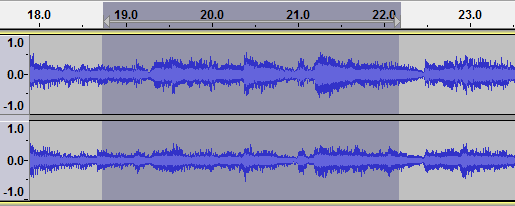
\includegraphics[max width=\linewidth]{../m/images/4/46/selected_audio_for_tour_guide.png}??
\textbf{Example of a stereo audio track with some audio selected - the selection is the dark gray section}

For more details on Play, Record and Edit see the Getting Started section of the Manual.
% <br/ title="Quick Help">



% <br/ title="Quick Help">

\section{Saving your work - audio formats}


\subsection{Save}


Audacity makes a distinction between saving audio in \textbf{Audacity project format} which only Audacity can open, and exporting audio in formats like WAV and MP3 for use in other applications. Audacity project format is made up of multiple small files which are stored in the \_data folder for the project and alongside that, an  AUP file which says what order the files are in. To reopen a saved project, open the AUP file, \textit{\textbf{not}} the multiple small files. 

\subsection{Export}


Use Export if you want to create a file in an audio format for playing outside of Audacity.
\begin{itemize}
\item  \textbf{LAME:} Do you want to convert a recording to compressed MP3 format? Audacity can, but it needs an add-on to do so.  The add-on is a library called \&lsquo;LAME\&rsquo;.  A free copy of LAME that is compatible with Audacity is available from the   lame.buanzo.org site, as per these instructions (Buanzo is a technology and security consultant from Argentina). 
\item  \textbf{FFmpeg:} The optional FFmpeg library allows Audacity to import and export a much larger range of audio formats including \textit{\textbf{M4A (AAC)}}, AC3, AMR (narrow band) and \textit{\textbf{WMA}}. Audacity can import audio from most video files by using FFmpeg.
\end{itemize}


% <br/ title="Glossary">

\section{Themes}


Audacity has four pre-configured, user-selectable, themes.  This enables you to choose the look and feel you prefer for Audacity's interface. see the Themes page for details.
\begin{itemize}
\item \textbf{Light} theme: this is a light theme loosely based on the look and feel of earlier Audacity versions, but given a contemporary twist with more modern-looking buttons and icons. 
\item \textbf{Dark} theme: created by the Dark Audacity project.\footnote{See URL http://www.darkaudacity.com/} This is similar to the Light theme, with the same buttons and icons, but given a dark twist.
\item \textbf{Classic} theme: The one you know and loved. This theme is a re-creation of the look and feel of earlier Audacity versions. 
\item \textbf{High Contrast} theme: some users with poor eyesight benefit from a high contrast that is 'eye-popping' for most people.
\end{itemize}

% <tbody rel="nofollow">
\* \* \* \* \includegraphics[max width=\linewidth]{../m/images/5/51/theme_light.png}
\* \* \* \* \includegraphics[max width=\linewidth]{../m/images/e/e3/theme_dark.png}
\* \* \* \* 
\textbf{Light} theme
\* \* \* \* 
\textbf{Dark} theme
% </tbody valign="top">

% <tbody valign="top">

\* \* \* \* \includegraphics[max width=\linewidth]{../m/images/b/bc/theme_classic.png}
\* \* \* \* \includegraphics[max width=\linewidth]{../m/images/c/c3/theme_hi_contrast.png}
\* \* \* \* 
\textbf{Classic} theme
\* \* \* \* 
\textbf{High Contrast} theme
% </tbody valign="top">



% <br/ valign="top">

\section{Faster ways to do things - shortcuts and Chains}

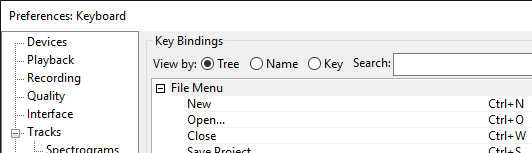
\includegraphics[max width=\linewidth]{../m/images/0/04/fragment_of_the_keyboard_preferences_dialog.png}\textbf{A fragment of the keyboard preferences dialog showing some shortcuts}

\subsection{Shortcuts}


Many buttons and menu commands have pre-defined keyboard shortcuts assigned.  You can modify these or add your own with Keyboard Preferences (in the Edit menu on Windows and Linux or the \texttt{{}"{}}Audacity\texttt{{}"{}} menu on Mac). 

\subsection{Chains}


Ever want to do the same thing to a large number of audio files, for example remove noise from them and convert to MP3?  Chains is the feature for this. Give it a list of files to work through and tell it what sequence of things to do. Programmers may want instead to use Scripting, an experimental but more flexible version of Chains. This needs a free experimental module called mod-script-pipe and experience in programming.

\subsection{Export Multiple}


You can save several audio files at once, rather than saving them one by one.


% <br/ title="Export Multiple">

\section{Changing the loudness of your audio - fades, Amplify, pan and gain}

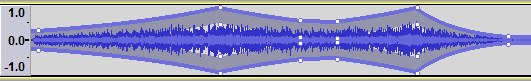
\includegraphics[max width=\linewidth]{../m/images/b/b0/a_small_image_of_an_envelope.png}\textbf{Mono track showing an amplitude Envelope}

\subsection{Amplify}


The \textbf{Amplify} audio effect makes audio louder or quieter.  Two other effects that modify loudness are \textbf{Fade In} and \textbf{Fade Out}.  These are often used at the beginning and end of audio. 
\begin{itemize}
\item  \textbf{Envelopes} provide a more flexible way to control loudness.  You will need to select the \textbf{Envelope Tool} or \textbf{Multi-Tool} to use envelopes.  With envelopes you can graphically control when audio gets louder and quieter.
\end{itemize}

\subsection{Pan and Gain}


These are the two sliders in the track's Track Control Panel. The \textbf{Gain} slider enables you to set the loudness for the track.  The \textbf{Pan} slider lets you make the audio louder on the left or the right. You can move these sliders to affect the audio as it plays.

\subsection{Mute and Solo}


These two buttons are in the track's Track Control Panel. Click the Mute button to silence this track when playing, click again to hear it again. Click the Solo button to play just this track. Click again to release the button. 

\subsection{Auto Duck}


This reduces (ducks) the volume of one or more selected tracks whenever the volume of a single unselected \texttt{{}"{}}control track\texttt{{}"{}} placed underneath reaches a particular threshold level. It can be used to create voice-overs for podcasts or DJ sets, for automatic \texttt{{}"{}}ramping\texttt{{}"{}} of background music in radio productions and for turning down a voice in original language as soon as its translation kicks in.

\subsection{Mixer Board}


An alternative view to the audio tracks in the main tracks window, and is analogous to a hardware mixer board. Each audio track is displayed in a Track Strip with its own pair of meters, gain slider, pan slider, and mute/solo buttons, mirroring that track's controls in its Track Control Panel. 


% <br/ title="Mixer Board">

\section{Noise in your audio - reducing, adding, fine tuning}

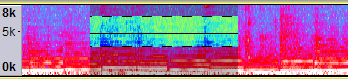
\includegraphics[max width=\linewidth]{../m/images/6/65/a_small_spectral_selection.png}\textbf{Mono track in Spectrogram view showing a Spectral Selection}

\subsection{Spectral Selection}


This is a special feature within \textbf{Sectrograms}, which lets you view the frequency content of audio then edit just selected frequencies.  This is particularly useful for voice recordings.  Among other purposes, Spectral Selection and editing can be used for cleaning up unwanted sound by removing particular frequencies, enhancing certain resonances, changing the quality of a voice or removing mouth sounds from voice work.

\subsection{Noise Reduction}


Audacity can remove some kinds of noise from a recording.  Noise Reduction is an \&lsquo;audio effect\&rsquo;, one of the fiddlier audio effects to use.  This effect works best with fairly constant noise like background hiss.  You first select audio that is just the noise and create a \&lsquo;noise profile\&rsquo;.  Once Audacity knows the noise profile, it can reduce the loudness of noise of that kind in audio you select. 

\subsection{Notch Filter}


This can be used to help you remove mains hum or electrical whistle with minimal damage to the remaining audio, by cutting a \texttt{{}"{}}notch\texttt{{}"{}} out of the frequency spectrum at that point.

\subsection{Generate Noise}


Audacity can add noise to a recording too. Three different types of noise can be generated. White noise has the greatest ability to mask other sounds, as it has similar energy at all frequency levels. If you want to add some room noise to make silences more realistic, try adding it at 0.001 amplitude.

\subsection{Draw Tool}


If you \textbf{Zoom} in enough on the audio you can edit individual samples of audio. Usually there are 44100 sample dots for every second of audio.  This  gives you an idea of how the audio is stored in the computer.  Very occasionally there may be a click in the audio which is better removed with Draw Tool than with \textbf{Click Removal} or the \textbf{Repair} effect.  Repair is best used when zoomed in a lot as it only works with short pieces of audio.


% <br/ title="Repair">

\section{Navigation and changing speed and pitch}


\includegraphics[max width=\linewidth]{../m/images/1/1f/transcription_toolbar_basic7.png}??\textbf{Transcription Toolbar}

\subsection{Play-at-speed}


Audacity has a \textbf{Transcription Toolbar} with a small button with green arrow pointing right, looking like the larger button with green arrow for \&lsquo;Play\&rsquo;.  Set the speed to go faster or slower using the slider to the right of the button.  You need to stop and restart playback for the new speed to happen. The speed change also changes the pitch.  This is a temporary change during playback.  To make a permanent change to speed and pitch use the Change Speed effect (below).

\subsection{Scrubbing and Seeking}


This is the action of moving the mouse pointer right or left so as to adjust the position, speed or direction of playback, forwards or backwards, listening to the audio at the same time - a convenient way to quickly navigate the waveform to find a particular event of interest. When Scrubbing or Seeking you can also use the mouse wheel to change the speed of the scrub or seek so this is another way to change playback speed.

\subsection{Change Speed, Change Pitch, Change Tempo}


You can speed audio up or slow it down by applying an effect that changes the audio:  
\begin{itemize}
\item  Use \textbf{Change Speed} to make audio faster or slower and higher or lower pitched. 
\item  Use \textbf{Change Pitch} to change the pitch of a selection without changing its tempo (speed). 
\item  Use \textbf{Change Tempo} if you want the pitch to stay the same when speeding up or slowing down. Change Tempo does not always work so well with large changes in speed and the end result may sound a little strange.
\end{itemize}

\subsection{Time Tracks}


A Time Track is a graph line you drag on to change the amount of speed-up or slow-down over time, instead of it having to be a constant speed change. As with Play-at-Speed the speed changes immediately without waiting to run an effect, but the changes do apply when exporting unless you delete the Time Track. So export a copy of your work to WAV format before using Time Track to be safe. 


% <br/ title="Time Tracks">

\section{Lots of things you might not know Audacity could do}

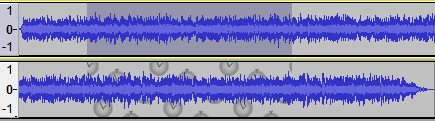
\includegraphics[max width=\linewidth]{../m/images/b/b7/a_small_image_of_sync_lock.png}??\textbf{A pair of Sync-Locked mono tracks: selection extends automatically to the second track}

\subsection{Sync-Lock}


When you have a mix (several tracks above each other which play together) and everything is nicely lined up, an edit in one track such as cutting a piece of audio can cause the mix to no longer to play in sync. To keep tracks aligned despite cutting, pasting or shifting audio, use Sync-Lock Tracks.

\subsection{Labels}


Use a Label Track to mark or annotate audio.  In conjunction with Sync-Lock you can keep the labels and audio in step.

\subsection{Undo and Redo}


These are most useful when working with effects.  After you have applied an effect you might change your mind.  The Undo button or menu item Edit \mbox{$>$} Undo will let you undo the change. The \textbf{History} menu item lets you look further back in time and undo more changes in one step.

\subsection{Truncate Silence}


A convenient effect to apply to recordings of interviews and speeches that removes long silences.  You can tell it what to count as a long silence, the loudness level and duration, and how much of each long silence to remove.

\subsection{Snap To}


When making selections it sometimes is helpful for the selection boundaries to be automatically moved to the nearest second (or some other unit of time measurement).  If you \&lsquo;snap-to\&rsquo; seconds your selections will always be whole numbers of seconds - you can\&rsquo;t select half a second of sound for example.  Set the time format to seconds or frames or whatever unit of time you want to snap to as well as enabling snap-to.

\subsection{Effects Plug-ins}


You can add to the effects available in Audacity using plug-ins.  Some of these have very nice looking interfaces with graphs and buttons and provide similar effects with different features, or effects that Audacity does not ship with. There are several types of plug-in. The \textbf{Nyquist} type of plug-in, for example, is Audacity's own plug-in format. Nyquist plug-ins can be made just by writing text in a file, so contributors to Audacity often use this format to create new effects. Thoroughly tested plug-ins are available from Download Nyquist Plug-ins. Experimental plug-ins, such as those for the hard task of removing pops, clicks and \texttt{{}"{}}ess\texttt{{}"{}} sounds from a voice recording, can be found on the Nyquist board on Audacity Forum.

\subsection{Multi-Clip}


Many people have a single piece of audio on each audio track.  However, you can have multiple pieces of non-overlapping audio on the same track.  These are called clips.  Clips can be created with \textbf{Split} and joined back together by clicking on the dark line boundary between clips. If you click the \textbf{Time Shift Tool} you can drag clips around to different positions on the track, or drag them to different tracks.%  
% NewPP limit report
% Cached time: 20171019095426
% Cache expiry: 86400
% Dynamic content: false
% CPU time usage: 0.159 seconds
% Real time usage: 0.168 seconds
% Preprocessor visited node count: 289/1000000
% Preprocessor generated node count: 561/1000000
% Post‐expand include size: 1512/2097152 bytes
% Template argument size: 876/2097152 bytes
% Highest expansion depth: 3/40
% Expensive parser function count: 0/100
% 
%  
% Transclusion expansion time report (%,ms,calls,template)
% 100.00%   19.060      1 - -total
%  28.26%    5.387      5 - Template:Key
%  14.49%    2.762      3 - Template:Button
%  10.72%    2.043      1 - Template:Intro
%   9.60%    1.830      1 - Template:Note
%   8.75%    1.667      2 - Template:Ednote
%   6.65%    1.268      1 - Template:Menu
% 
%  Saved in parser cache with key helpmediawiki:pcache:idhash:5534-0!*!0!!*!5!* and timestamp 20171019095426 and revision id 55397
%  

										%  end content 
																					%  end of the left (by default at least) column 
											
% html: End of file: `audacity_tour_guide.html'

\iffalse
\label{newXfeaturesXinXthisXreleaseX}
\ensurespace\section{New features in this release}
\par\vspace{1mm}\hrule
\begin{multicols}{2}\par \protect
\includegraphics[max width=\linewidth]{C:/OpenSourceGit/AudacityTeamTools/test/m/images/8/88/audacity_logo_signika_512_transparent.png}\par \textbf{This page is an overview of the key new functionality that has been introduced in Audacity 2.2.0}
\begin{itemize}
\item Details of all the major changes since 2.1.3 can be found in Release Notes 2.2.0.
\end{itemize}

\label{newXfeaturesXinXthisXreleaseXlogo}
\subsection{New Logo}The logo has been given a refresh, and now uses a sans-serif font and a flatter style.
\par \protect
\includegraphics[max width=\linewidth]{C:/OpenSourceGit/AudacityTeamTools/test/m/images/8/8c/audacity_logo_whitebg.png}\par 
\label{newXfeaturesXinXthisXreleaseXthemes}
\subsection{
\hyperref[\foo{themesX}]{Themes}
}Audacity now comes supplied with four pre-configured, user-selectable, themes.  This enables you to choose the look and feel you prefer for Audacity's interface. see the 
\hyperref[\foo{themesX}]{Themes}
 page for details.

\begin{itemize}
\item \textbf{Light} theme: this is a light theme loosely based on the look and feel of earlier Audacity versions, but given a contemporary twist with more modern-looking buttons and icons. 
\item \textbf{Dark} theme: created by the Dark Audacity project. This is similar to the Light theme, with the same buttons and icons, but given a dark twist.
\item \textbf{Classic} theme: The one you know and loved. This theme is a re-creation of the look and feel of earlier Audacity versions. 
\item \textbf{High Contrast} theme: some users with poor eyesight benefit from a high contrast that is 'eye-popping' for most people.
\end{itemize}
\par \protect\includegraphics[max width=\linewidth]{C:/OpenSourceGit/AudacityTeamTools/test/m/images/5/51/theme_light.png}\par \par \protect\includegraphics[max width=\linewidth]{C:/OpenSourceGit/AudacityTeamTools/test/m/images/e/e3/theme_dark.png}\par \textbf{Light} theme
\textbf{Dark} theme
\par \protect\includegraphics[max width=\linewidth]{C:/OpenSourceGit/AudacityTeamTools/test/m/images/b/bc/theme_classic.png}\par \par \protect\includegraphics[max width=\linewidth]{C:/OpenSourceGit/AudacityTeamTools/test/m/images/c/c3/theme_hi_contrast.png}\par \textbf{Classic} theme
\textbf{High Contrast} theme
The theme to use can be chosen at Edit > Preferences > 
\hyperref[\foo{interfaceXpreferencesX}]{Interface}
.  

\begin{itemize}
\item  In addition to the four pre-configured themes there is also a Custom theme.  
\end{itemize}
 By default the custom theme looks the same as Classic theme - but, if you have the right programming skills and tools, you can use this template to create your own theme.  Instructions for how to do this may be found in the Audacity Wiki.
\label{newXfeaturesXinXthisXreleaseXmidi}
\subsection{MIDI (and Allegro) Playback}Playback of MIDI (and Allegro) files imported into 
\hyperref[\foo{noteXtracksX}]{Note Tracks}
 is now available.  Please see the 
\hyperref[\foo{noteXtracksX}]{Note Tracks}
 page for more details.
This should just work on Windows but for playback on Mac and Linux additional software may be required, see 
\hyperref[\foo{playingXandXrecordingXmidi}]{this section}
 on the 
\hyperref[\foo{playingXandXrecordingX}]{Playing and Recording}
 page.
But note that there will no use of the 
\hyperref[\foo{meterXtoolbarXplayback}]{Playback meter}
 while Note tracks are played. 

\label{newXfeaturesXinXthisXreleaseXstemplots}
\subsection{Stem Plots}There is a new entry in the 
\hyperref[\foo{tracksXpreferencesX}]{Tracks Preferences}
 for \textbf{Display samples}.  This setting changes how 
\hyperref[\foo{audacityXwaveformX}]{Waveform}
 and 
\hyperref[\foo{audacityXwaveformXdb}]{Waveform dB}
 views are displayed.  It only affects the appearance of the waveform when you are so far zoomed in that you can see the individual sample dots.  At lower zoom levels it makes no difference.  

\begin{itemize}
\item \textbf{Stem plot:} This is the default setting which draws a vertical line from the track center line to the sample dot, giving a clearer impression of the relative amplitude of the samples. As seen in the images below, when zoomed out close to the minimum for a stem plot, the horizontal distance between sample dots may be more uneven than seen with the connect dots default.   
\item \textbf{Connect dots:} This is alternative setting yields a waveform where each sample dot is connected to the next sample by a line drawn between them.  
\end{itemize}
\par \protect\includegraphics[max width=\linewidth]{C:/OpenSourceGit/AudacityTeamTools/test/m/images/e/ef/connect_dots_stem_plot_examples.png}\par Uneven spacing is due to "aliasing", but zooming in further will equalize the spacing whether choosing Connect dots or Stem plot.
\label{newXfeaturesXinXthisXreleaseXmenus}
\subsection{Menu reorganization}We have made the Menus shorter and clearer than in previous Audacity versions. The menus have been simplified without losing functionality. The most commonly used functions are found in the top levels of the menus. The functions moved down into lower submenus are better organized.
This is not just a rearrangement.  We also added new menu items to make the layout more logical.  There are new menu items for exporting as MP3 or WAV. Previously you had to export audio, and then choose the format. You still can do that, but these new items are there for convenience.
One of the long standing bug-bears with Audacity is the distinction between ‘Save’ and ‘Export’. People expect to be able to open a WAV audio file, edit it in Audacity and then click save. That is not how Audacity works. Audacity needs audio in its own unique format to work on it. So Audacity converts when you 'Open' a WAV file and converts back when you 'Save'. In an attempt to make this clearer Audacity uses the word 'Import' for opening a file like WAV and 'Export' for converting and saving in a format like WAV. Open and Save are reserved for Audacity's own project format.Now the ‘Export’ options are under the ‘Save Other’ menu item, where people trying to save audio as an MP3 or WAV file are more likely to find them.
\label{newXfeaturesXinXthisXreleaseXextendedmenubar}
\subsection{The Extended Menu bar}There are two new additional menus that are hidden by default.  They can be turned on at View > 
\hyperref[\foo{viewXmenuXextraXmenusXonoff}]{Extra Menus (on/off)}
 or the Interface pane of Edit > 
\hyperref[\foo{interfaceXpreferencesX}]{Preferences}
.
These extra menus have many extra less frequently used commands.  They are particularly useful to VI users, but normally-sighted users may find them useful too.
\textit{\textbf{Image of the Extended Menu bar as it appears on Windows}}\par \protect\includegraphics[max width=\linewidth]{C:/OpenSourceGit/AudacityTeamTools/test/m/images/0/0d/menu_toolbar_extra.png}\par \textit{Click, or hover, on either of the \textbf{Ext-} items at the end of the image to read about those menu entries.}Menu
What you'll find there

\hyperref[\foo{extXbarXmenuX}]{Ext-Bar}
The Ext-Bar menu provides access to 
\hyperref[\foo{toolbarsXoverviewX}]{Toolbar}
 operations that are not available in the default Audacity menus. These will be of most interest to visually impaired users or those who have difficulty using the mouse.
\hyperref[\foo{keyboardXpreferencesX}]{Shortcuts}
 can be assigned to these commands if required.
\hyperref[\foo{extXcommandXmenuX}]{Ext-Command}
The Ext-Command menu provides access to extra commands for 
\hyperref[\foo{audioXtracksXfocus}]{track focus}
 and movement of the editing or playback cursor that are not available in the default Audacity menus. These will be of most interest to visually impaired users or those who have difficulty using the mouse.
\hyperref[\foo{keyboardXpreferencesX}]{Shortcuts}
 can be assigned to these commands if required.If you only require regular access to a small set of these commands you can set shortcuts for them and leave the extra menus hidden.
\label{newXfeaturesXinXthisXreleaseXappend}
\subsection{Appended recording on the same track in now the default}From Audacity 2.2.0 onward the default recording mode has changed so that when you click the Record button \protect
\includegraphics[max width=\linewidth]{C:/OpenSourceGit/AudacityTeamTools/test/m/images/e/e8/record.png} on 
\hyperref[\foo{transportXtoolbarX}]{Transport Toolbar}
, or use the R, Audacity will record at the end of the currently selected (or only) track.

\subsubsection{To record on a new track}If you hold the Shift button down the Record button in 
\hyperref[\foo{transportXtoolbarX}]{Transport Toolbar}
 will temporarily change to \protect
\includegraphics[max width=\linewidth]{C:/OpenSourceGit/AudacityTeamTools/test/m/images/7/72/record_new_track.png}. Then clicking on this modified Record button, or using the shortcut Shift + R will cause Audacity to create a new track and begin recording on that track from the current cursor position (or from the left edge of a region on the 
\hyperref[\foo{timelineX}]{Timeline}
). 

\label{newXfeaturesXinXthisXreleaseXhelp-buttons}
\subsection{Help buttons}Many places in the user interface have had a help button \protect
\includegraphics[max width=\linewidth]{C:/OpenSourceGit/AudacityTeamTools/test/m/images/d/d6/help_button.png} added. Examples are all the Preferences dialog panes, all the Effects, Generators and Analyzers and some error messages.
Clicking on that button in the dialog will link you to the appropriate page in the Manual.
Example: the Amplify effect.  Try clicking on the "\textbf{?}" at the bottom right of this image.
\par \protect\includegraphics[max width=\linewidth]{C:/OpenSourceGit/AudacityTeamTools/test/m/images/6/6d/amplify.png}\par 
\label{newXfeaturesXinXthisXreleaseXshortcuts}
\subsection{Standard and Full shortcut sets}For Audacity 2.2.0 we have reduced the number of preset shortcuts in the application to a "\textbf{
\hyperref[\foo{keyboardXshortcutXreferenceX}]{Standard}
}" set.  We did this to simplify the set of shortcuts somewhat and to provide greater flexibility for users who want to set their own custom shortcuts.
You can choose to revert to the full set of shortcuts that were in 2.1.3 and earlier by selecting "\textbf{Full}" from the dropdown menu accessed from the Defaults button in the 
\hyperref[\foo{keyboardXpreferencesX}]{Keyboard Preferences}
 dialog.
You can use the Defaults button to switch between the two provided default sets of shortcuts at any time.
\par \protect\includegraphics[max width=\linewidth]{C:/OpenSourceGit/AudacityTeamTools/test/m/images/f/f8/preferences_keyboard_with_default_dropdown_menu_trimmed.png}\par See 
\hyperref[\foo{keyboardXshortcutXreferenceX}]{Commands and Keyboard Shortcut Reference}
 for more details.

\label{newXfeaturesXinXthisXreleaseXselection}
\subsection{Selection Toolbar improvements}There are now four available settings in the Selection and Audio Position Boxes in 
\hyperref[\foo{selectionXtoolbarX}]{Selection Toolbar}
 for the  manner in which the details of your selection are displayed:

\begin{itemize}
\item \textbf{Start and End of selection}: the start time and the end time of your selection \textit{(default setting)}
\item \textbf{Start and Length of selection}: the start time and the length of your selection
\item \textbf{Length and End of selection}: the length and the end time of your selection
\item \textbf{Length and Center of selection}: the length and the time at the center of your selection
\end{itemize}
\par \protect\includegraphics[max width=\linewidth]{C:/OpenSourceGit/AudacityTeamTools/test/m/images/c/c6/selection_toolbar_display_modes.png}\par 
\label{newXfeaturesXinXthisXreleaseXclips}
\subsection{New commands for using clips via the keyboard}New commands, all of which interact with the clips on the focused track. As yet, there are no default shortcuts:

\begin{enumerate}
\item Transport > Cursor to > 
\hyperref[\foo{transportXmenuXcursorXtoXpreviousXclipXboundary}]{Previous clip boundary}

\item Transport Cursor to > 
\hyperref[\foo{transportXmenuXcursorXtoXnextXclipXboundary}]{Next clip boundary}

\item Select > Clip Boundaries > 
\hyperref[\foo{selectXmenuXclipXboundariesXpreviousXclipXboundaryXtoXcursor}]{Previous clip boundary to cursor}

\item Select > Clip Boundaries > 
\hyperref[\foo{selectXmenuXclipXboundariesXcursorXtoXnextXclipXboundary}]{Cursor to next clip boundary}

\item Select > Clip Boundaries > 
\hyperref[\foo{selectXmenuXclipXboundariesXpreviousXclip}]{Previous clip}

\item Select > Clip Boundaries > 
\hyperref[\foo{selectXmenuXclipXboundariesXnextXclip}]{Next clip}

\end{enumerate}
There are also two new commands (
\hyperref[\foo{extXcommandXmenuXcursorXclipXleft}]{Clip Left}
 and 
\hyperref[\foo{extXcommandXmenuXcursorXclipXright}]{Clip Right}
) for moving clips, which are available in the 
\hyperref[\foo{newXfeaturesXinXthisXreleaseXXextendedmenubar}]{extended menus}
 added in this release.Note that these extended menus are \textit{\textbf{not}} turned on by default, to turn them on please see 
\hyperref[\foo{menuXreferenceXtheXextendedXmenuXbar}]{Menu Reference}
 for how to reveal the extended menus.
\label{newXfeaturesXinXthisXreleaseXsafety}
\subsection{Running out of disk space}We have now provided an error trap for situations where you are running out of available disk space.
You will now see the error message:
"\textbf{Audacity failed to write to a file in <device>}"
This is particularly useful when recording as Audacity will stop recording when the error is trapped, preserving your recording up to that point.

\label{newXfeaturesXinXthisXreleaseXappendix}
\subsection{
\hyperref[\foo{newXfeaturesXinXthisXreleaseXappendixX}]{Additional new features}
}This page \textbf{
\hyperref[\foo{newXfeaturesXinXthisXreleaseXappendixX}]{New features in this release - appendix}
} gives an overview of further new functionality that has been introduced in this release of Audacity.

\subsection{Links}\textbf{>} Audacity Release Notes 2.2.0\textit{- detailed release notes for this release of Audacity}\end{multicols}
\input{./man/audacity_tour_guide.tex}
\fi

\end{document}
